%!TEX root = Thesis.tex

\chapter{Coordination Complexes with Rhodium and Iridium}
\chaptermark{Rhodium and Iridium}
\label{ch:rhodium}

The xantphos class of ligands were first studied for their potential use as ancillary ligands in rhodium catalysed hydroformylation\cite{Kranenburg1995}.  It was found increasing the bite-angle from 108.7\degrees for sixantphos to 109.4 \degrees for thixantphos and 111.7 \degrees for xantphos resulted in an increase in the selectivity for the linear aldehyde (linear/branched = 35.0, 47.6 and 57.1 respectively).  A more recent paper with \iPrxantphos{} found a dramatic difference between the reactivity of the diphosphine towards rhodium and iridium.  Studying the coordination behaviour of the \tBuxantphos{} ligands with rhodium and iridium thus made logical sense.\fixme{scientific language!}

\section{Rhodium Complexes}
\label{section:experimental:rhodium}

Reaction between \ce{[Rh(COE)2Cl]2} and the diphosphines was carried out on an NMR scale in \ce{C6D6}.  A reaction occurs rapidly with all three diphosphine to form complexes \fixme{compound reference} (Scheme \ref{RhodiumI}).  These complexes have \JRhP{} coupling constants of around 142 Hz, consistent with rhodium(I).  The complexes are direct analogues of those reported for \iPrxantphos{} which has a \JRhP{} coupling constant of 142.4 Hz.\cite{Esteruelas2013}  The \tBuxantphos ligands are coordinated in a tridentate manner with the oxygen binding.  In the \carbon{} NMR spectrum this can be seen as the O-ipso carbon carbon has shifted to downfield.  For example in \tBuxantphos{} this carbon resonants at 155.8 ppm, in the complex \ce{[(tBu-xantphos)AgCl]} the carbon shifted to 156.5 although the oxygen was not binding.  In the tridentate rhodium complex this carbon has moved downfield again to 158.9 ppm.  This shift in the resonant frequency of this carbon is a result of the oxygen donating electron density to the rhodium, which in turn makes the oxygen withdraw electron density from the ipso carbons.  

\begin{scheme}[h]
\begin{center}
\vspace{0.5cm}
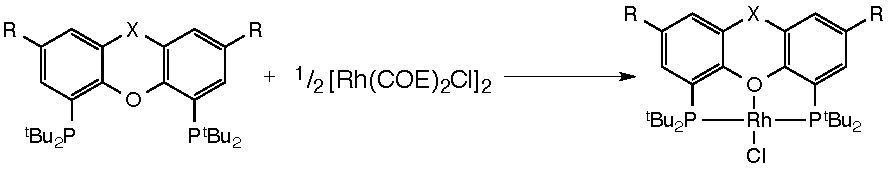
\includegraphics{../Schemes/RhodiumI.pdf}
\caption[Reaction of \ce{[Rh(COE)2Cl]2} and \tBuxantphos{} ligands]{Reaction of \ce{[Rh(COE)2Cl]2} and \tBuxantphos{} ligands.  \tBuxantphos: R = H, X = \ce{CMe2}. \tButhixantphos: R = Me, X = S. \tBusixantphos: R = H, X = \ce{SiMe2}}
\vspace{0.2cm} 
\label{RhodiumI}
\end{center}
\end{scheme}
\vspace{0.2cm}

Unlike the complexes with iPr-xantphos the complexes \ce{[Rh($\eta^3-$tBu-xantphos)Cl]} were unstable in solution over prolonged periods.  Overnight a new resonance appeared in the \phosphorus NMR spectrum, shifted upfield with a much smaller coupling constant (\JRhP{} = 101.5 Hz).  This decrease in coupling constant is consistent with an increase in the oxidation state to rhodium(III).  However, this occurred in dry, degassed\ce{C6D6} which should not be reactive towards the complex.  No signals other than those expected for the ligand were observed in the \proton, \carbon, or \phosphorus{} NMR spectra.  

Dark red crystals were obtained by slow evaporation of a benzene solution of the unknown rhodium(III) complex.  The crystal structure (Figures \ref{Crystal:rhodium} and \ref{Crystal:rhodiumside}) revealed the presence of a coordinated dioxygen molecule.  The complex crystallised as \ce{[Rh(tBu-xantphos)Cl(}$\eta_2$\ce{-O2})] in the orthorhombic space group \emph{Pbca}.  Selected bond lengths and angles are given in Table \ref{crystal:rhodium:lengths} and crystallographic data is given in Table \ref{crystal:rhodium:data}.  This complex likely formed by slow diffusion of oxygen through the septum sealing the NMR tube.  The crystal structure showed some substitutional disorder with the peroxo ligand substituted for an oxo ligand in approximately 15\% of the sites.  Selected bond lengths and angles for the oxo complex are given in Table \ref{crystal:rhodium:lengths:oxo}.

\begin{figure}[htp]
\begin{center}
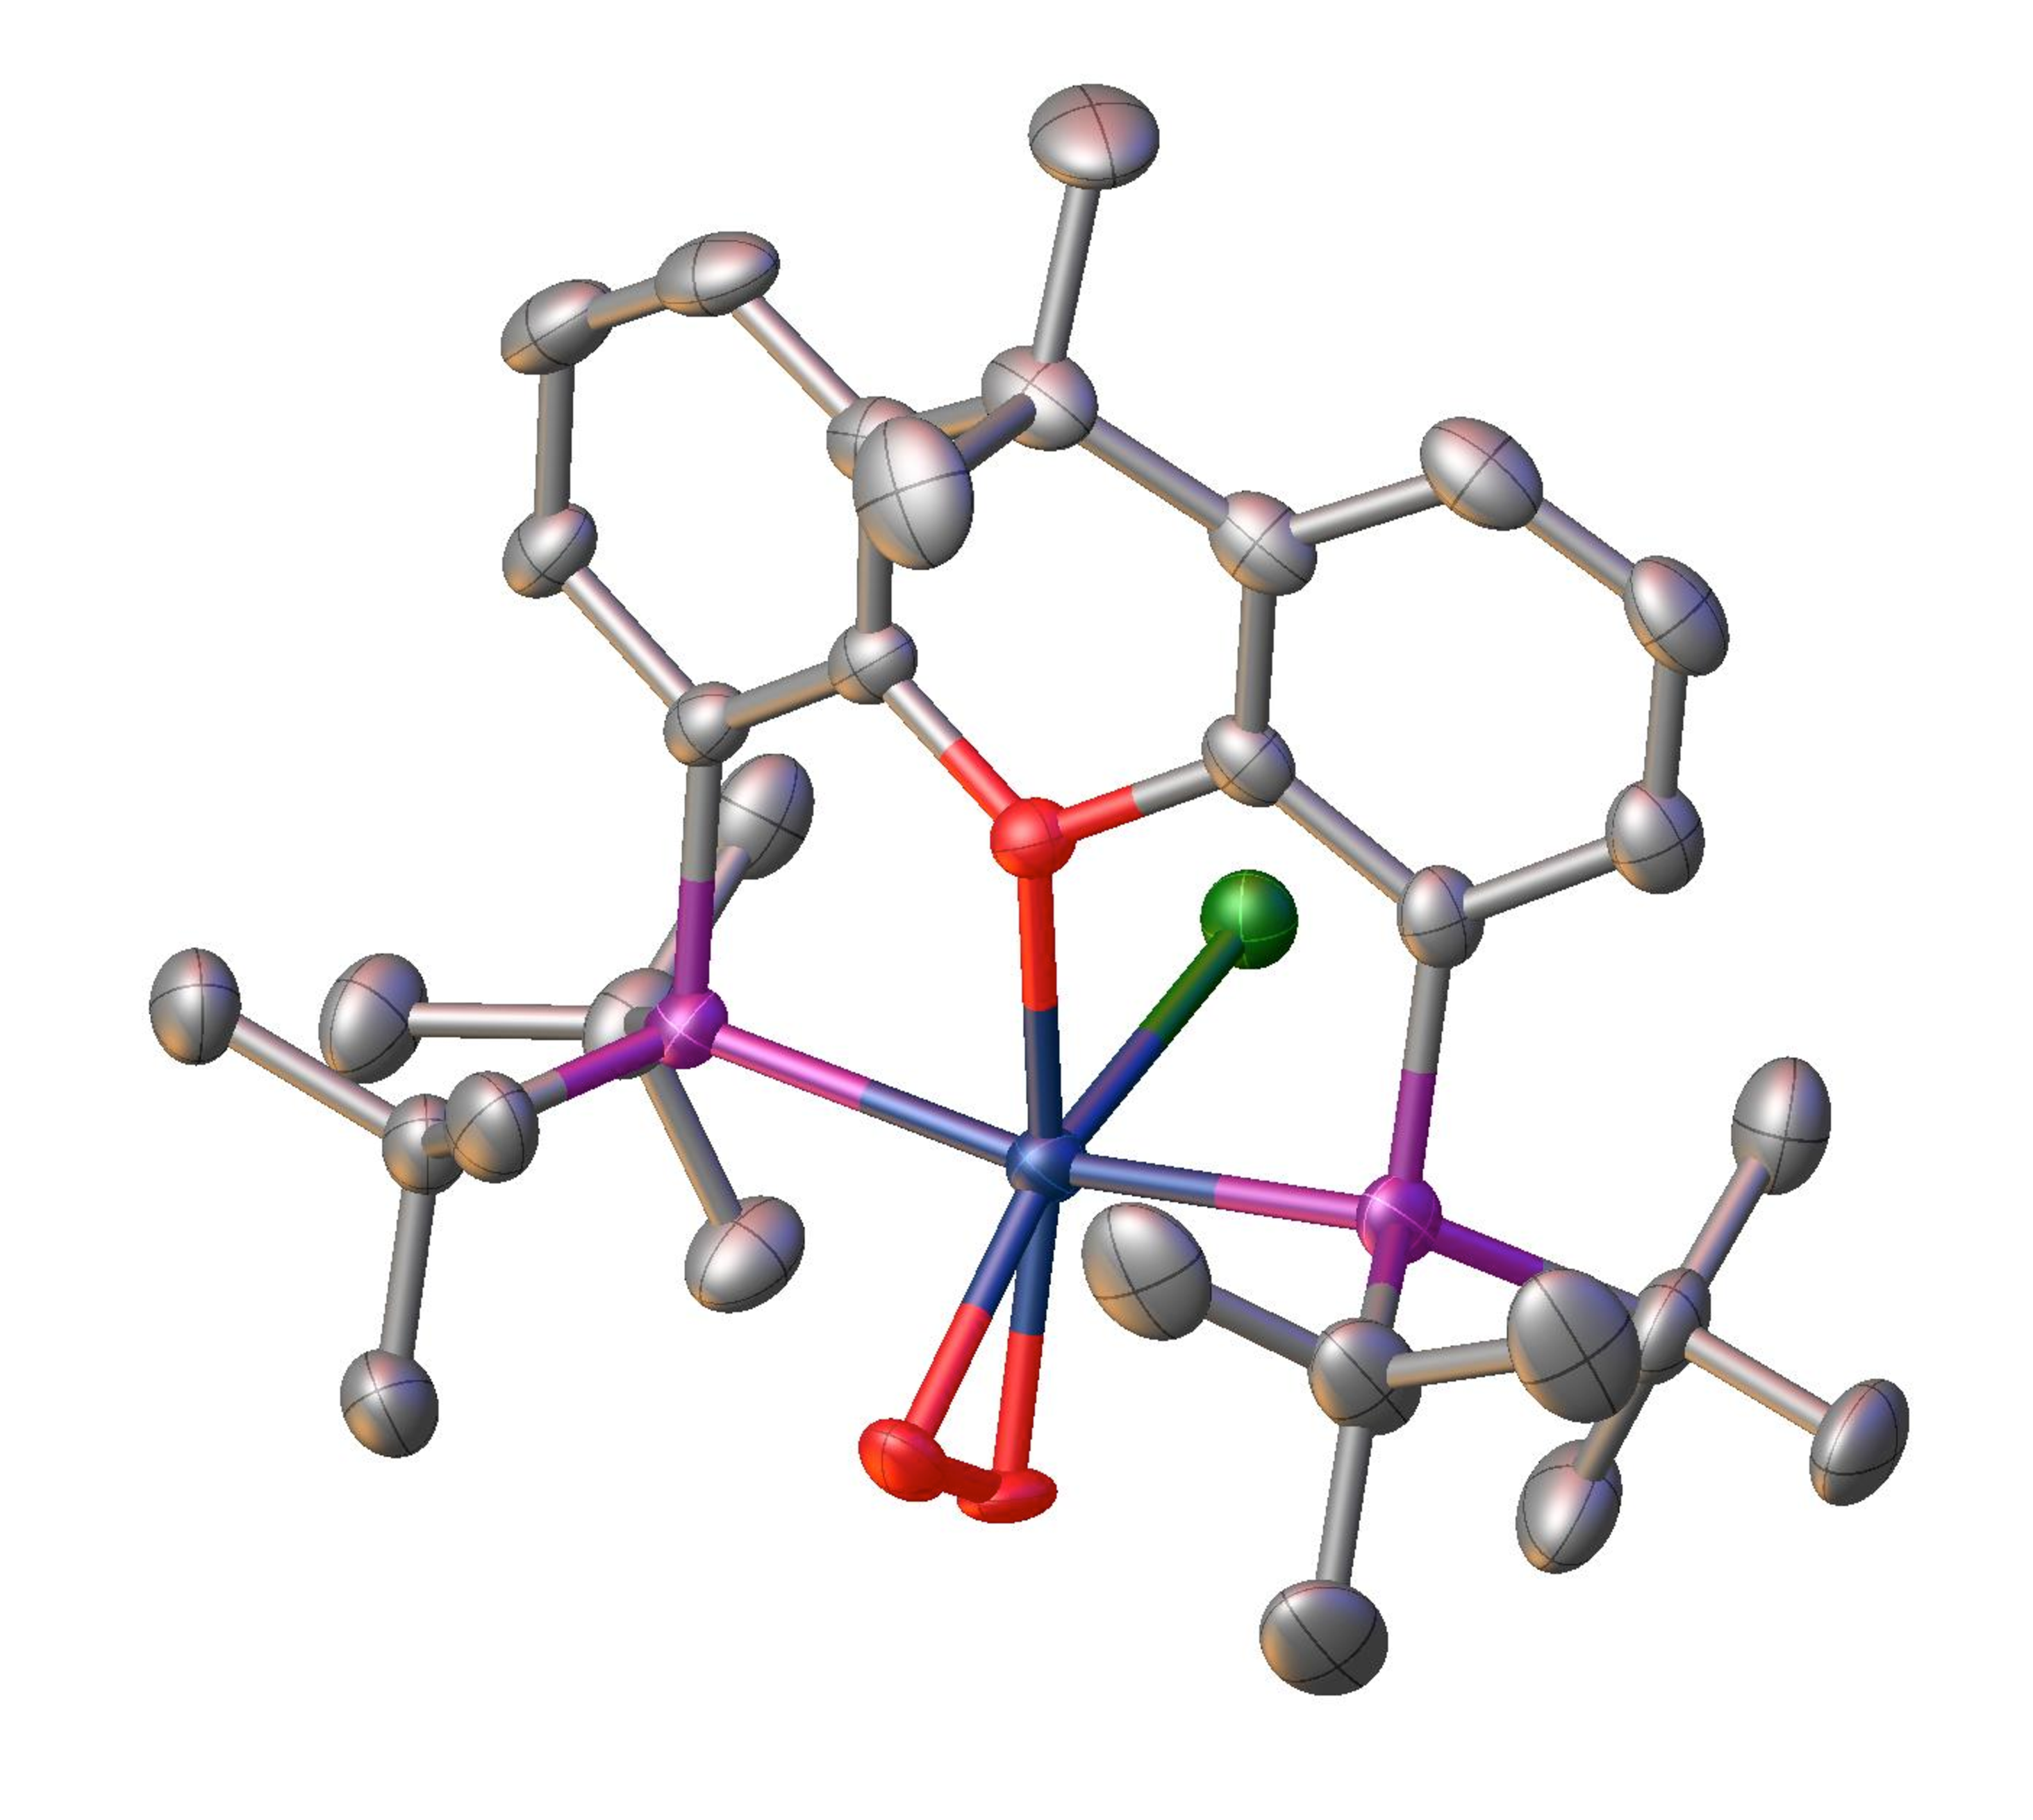
\includegraphics[width=0.6\textwidth]{../Figures/Crystalrhodium.pdf}
\caption[X-ray crystal structure of \ce{[Rh(tBu-xantphos)Cl(}$\eta^2$\ce{-O2}){]}]{X-ray crystal structure of \ce{[Rh(tBu-xantphos)Cl(}$\eta^2$\ce{-O2})], hydrogen atoms omitted for clarity.}
\label{Crystal:rhodium}
\end{center}
\end{figure}

\begin{figure}[htp]
\begin{center}
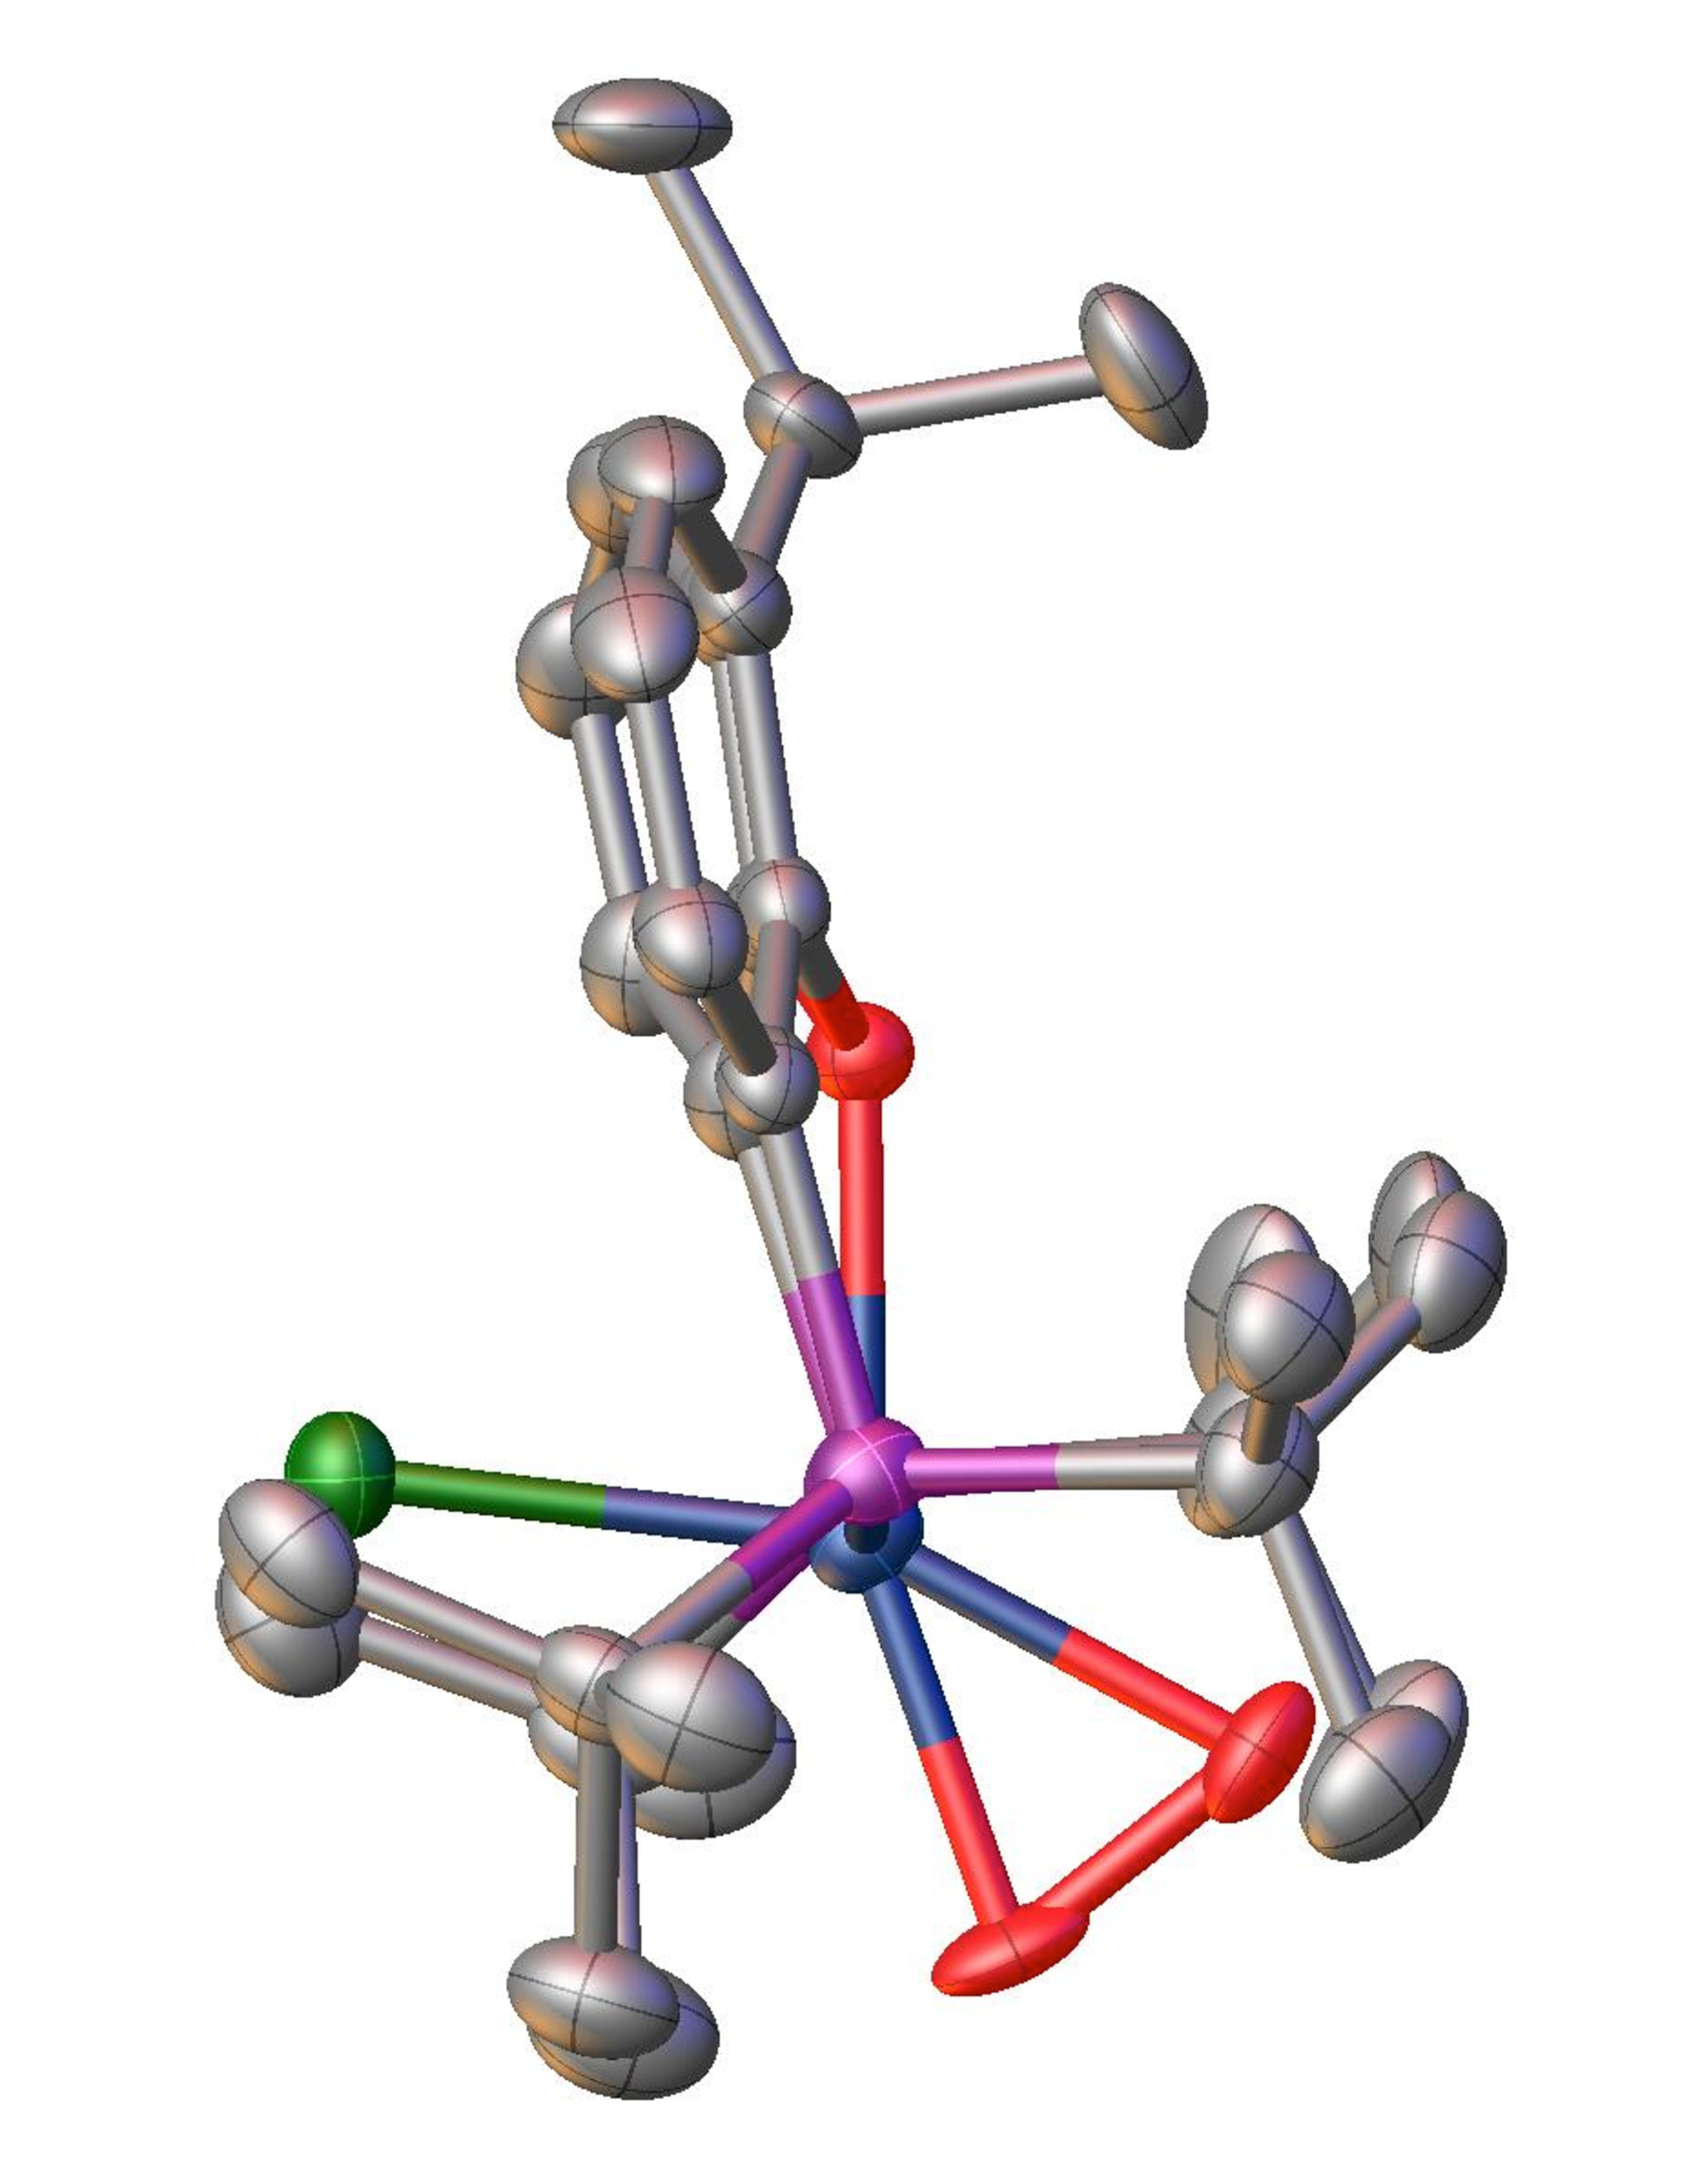
\includegraphics[width=0.4\textwidth]{../Figures/Crystalrhodiumside.pdf}
\caption[X-ray crystal structure of \ce{[Rh(tBu-xantphos)Cl(}$\eta^2$\ce{-O2}){]} - side view]{X-ray crystal structure of \ce{[Rh(tBu-xantphos)Cl(}$\eta^2$\ce{-O2})], hydrogen atoms omitted for clarity - side view}
\label{Crystal:rhodiumside}
\end{center}
\end{figure}

\begin{table}[htp]
\caption[Selected bond distances (\AA) and angles (\degrees) of \ce{[Rh(tBu-xantphos)Cl(}$\eta^2$\ce{-O2}){]}]{Selected bond distances (\AA) and angles (\degrees) of \ce{[Rh(tBu-xantphos)Cl(}$\eta^2$\ce{-O2})]}
\label{crystal:rhodium:lengths}
\begin{center}
\begin{tabular}{l l l l}
	\toprule
	\multicolumn{2}{l}{\bfseries{~Bond distances (\si{\angstrom})}} & \multicolumn{2}{c}{\bfseries{Bond angles (\degrees)}} \\
	\midrule		
%	~P1-O2		~~&~~XXXX~~	&~~					&~~XXXX~~	\\
%	~P1-O2		~~&~~XXXX~~	&~~					&~~XXXX~~	\\
%	~P1-O2		~~&~~XXXX~~	&~~					&~~XXXX~~	\\
%	~P1-O2		~~&~~XXXX~~	&~~					&~~XXXX~~	\\
%	~P1-O2		~~&~~XXXX~~	&~~					&~~XXXX~~	\\
%	~P1-O2		~~&~~XXXX~~	&~~					&~~XXXX~~	\\
%	~P1-O2		~~&~~XXXX~~	&~~					&~~XXXX~~	\\
	~O1-Pt		~~&~~3.565~~	&~~Ring 1-Ring 2		&~~XXXX~~		\\
	~O2-Pt		~~&~~3.497~~	&~~Ring 3-Ring 4		&~~XXXX~~		\\
%	~P1-O2		~~&~~XXXX~~	&~~					&~~XXXX~~	\\
%	~P2-O2		~~&~~XXXX~~	&~~					&~~XXXX~~	\\
%	~P3-O1		~~&~~XXXX~~	&~~					&~~XXXX~~	\\
%	~P4-O1		~~&~~XXXX~~	&~~					&~~XXXX~~	\\
	\bottomrule{}
\end{tabular}
\end{center}
\end{table}

\begin{table}[htp]
\caption[Selected bond distances (\AA) and angles (\degrees) of \ce{[Rh(tBu-xantphos)(O)Cl}{]}]{Selected bond distances (\AA) and angles (\degrees) of \ce{[Rh(tBu-xantphos)(O)Cl]}}
\label{crystal:rhodium:lengths:oxo}
\begin{center}
\begin{tabular}{l l l l}
	\toprule
	\multicolumn{2}{l}{\bfseries{~Bond distances (\si{\angstrom})}} & \multicolumn{2}{c}{\bfseries{Bond angles (\degrees)}} \\
	\midrule		
%	~P1-O2		~~&~~XXXX~~	&~~					&~~XXXX~~	\\
%	~P1-O2		~~&~~XXXX~~	&~~					&~~XXXX~~	\\
%	~P1-O2		~~&~~XXXX~~	&~~					&~~XXXX~~	\\
%	~P1-O2		~~&~~XXXX~~	&~~					&~~XXXX~~	\\
%	~P1-O2		~~&~~XXXX~~	&~~					&~~XXXX~~	\\
%	~P1-O2		~~&~~XXXX~~	&~~					&~~XXXX~~	\\
%	~P1-O2		~~&~~XXXX~~	&~~					&~~XXXX~~	\\
	~O1-Pt		~~&~~3.565~~	&~~Ring 1-Ring 2		&~~XXXX~~		\\
	~O2-Pt		~~&~~3.497~~	&~~Ring 3-Ring 4		&~~XXXX~~		\\
%	~P1-O2		~~&~~XXXX~~	&~~					&~~XXXX~~	\\
%	~P2-O2		~~&~~XXXX~~	&~~					&~~XXXX~~	\\
%	~P3-O1		~~&~~XXXX~~	&~~					&~~XXXX~~	\\
%	~P4-O1		~~&~~XXXX~~	&~~					&~~XXXX~~	\\
	\bottomrule{}
\end{tabular}
\end{center}
\end{table}

\begin{table}[htp]
\caption[Crystallographic data of \ce{[Rh(tBu-xantphos)Cl(}$\eta^2$\ce{-O2}){]}]{Crystallographic data of \ce{[Rh(tBu-xantphos)Cl(}$\eta^2$\ce{-O2}){]}} 
\label{crystal:rhodium:data}
\begin{center}
\begin{tabular}{l l}
	\toprule
	~~\bfseries{Empirical formula}~~&~~\fixme{XXXXX}\\
	\midrule	
	~~Formula weight~~		&~~XXX~~	\\
	~~Crystal system~~		&~~XXX~~	\\
	~~Space group~~		&~~XXX~~	\\
	~~a$/$\si{\angstrom}~~	&~~XXX~~	\\
	~~b$/$\si{\angstrom}~~	&~~XXX~~	\\
	~~c$/$\si{\angstrom}~~	&~~XXX~~	\\
	~~$\alpha/$\degrees~~	&~~XXX~~	\\
	~~$\beta/$\degrees~~	&~~XXX~~	\\
	~~$\gamma/$\degrees~~	&~~XXX~~	\\
	~~V$/$\si{\angstrom\cubed}&~~XXX~~	\\
	~~Z					&~~XXX~~	\\
	~~Cell determination reflections &~~XXX~~	\\
	~~Cell determination range, $\theta{}$\sub{min} $\longrightarrow \theta{}$\sub{max}/\degrees &~~XXX~~	\\
	~~Temperature $/$\si{\kelvin}	&~~XXX~~	\\
	~~Radiation type			&~~XXX~~	\\
	~~Radiation ($\lambda$) $/$\si{\angstrom}	&~~XXX~~	\\
	~~Crystal size $/$\si{\milli\metre}			&~~XXX~~	\\
	~~D\sub{\emph{calc}} $/$ \si{\gram\per\metre\cubed}	&~~XXX~~	\\
	~~F(000)				&~~XXX~~	\\
	~~$\mu /$	\si{\per\milli\metre}		&~~XXX~~	\\
	~~Experimental absorption correction type	&~~XXX~~	\\
	~~T\sub{max}, T\sub{min}	&~~XXX~~	\\
	~~Reflections collected					&~~XXX~~	\\
	~~Index range \emph{h}		&~~XXX~~	\\
	~~Index range \emph{k}		&~~XXX~~	\\
	~~Index range \emph{l}		&~~XXX~~	\\
	~~$\theta$ range $/$\degrees	&~~XXX~~	\\
	~~Independent reflections		&~~XXX~~	\\
	~~Reflections $[\emph{I} > 2\sigma(\emph{I})]$	&~~XXX~~	\\
	~~Restraints $/$ parameters	&~~XXX~~	\\
	~~GOF					&~~XXX~~	\\
	~~R\sub{1} $[\emph{I} > 2\sigma(\emph{I})]$	&~~XXX~~	\\
	~~wR2 $[\emph{I} > 2\sigma(\emph{I})]$	&~~XXX~~	\\
	~~R\sub{1} [all data]	&~~XXX~~	\\
	~~wR2 [all data]			&~~XXX~~	\\
	~~Residual density $/$e \si{\per\angstrom\cubed}	&~~XXX~~	\\
	\bottomrule{}
\end{tabular}
\end{center}
\end{table}


The complex shows two distinct methyl environments in the \proton{} and \carbon{} NMR spectra.\fixme{give values?}  This indicates a loss of symmetry across the two faces of the ligand.  From the crystal structure we can clearly see that the chloride ligand sits on the same side as the concave face of the ligand while the peroxo ligand occupies the position pseudo-\emph{trans} to the oxygen bridge of the ligand.  This geometry leaves more space \emph{trans} to the chloride resulting in the curvature of the ligand to occupy this free space and the tipping of the methyl groups away from the chloride.

The oxo complex shows a slightly distorted square-based pyramid structure with the ether bridge of the \tBuxantphos ligand occupying the apex.  To the best of our knowledge this is the first example of crystallographic evidence for a rhodium oxo complex.  The rhodium oxo bond is much shorter than the rhodium peroxo bond lengths consistent with the higher bond order.  The rhodium oxo complex was subsequently synthesis by reaction of the rhodium dioxygen complex with the rhodium(I) chloride complex.  The two complexes likely form a dimeric structure  with two bridging $\mu_2$  - oxo ligands, which then rearranges to give two rhodium oxo complexes (Figure \ref{Rhodiumrearrangement}).

\begin{scheme}[h]
\begin{center}
\vspace{0.5cm}
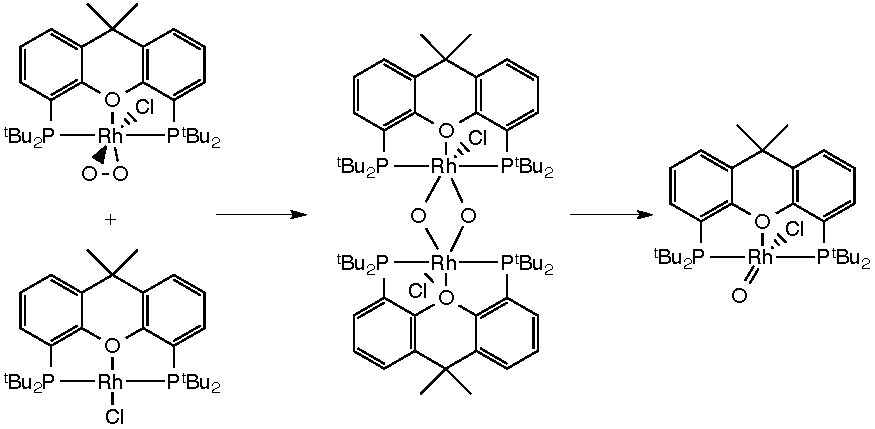
\includegraphics{../Schemes/Rhodiumrearrangement.pdf}
\caption[Formation of the rhodium oxo complex]{Formation of the rhodium oxo complex}
\vspace{0.2cm} 
\label{Rhodiumrearrangement}
\end{center}
\end{scheme}
\vspace{0.2cm}

The complexes \ce{[Rh($\eta^3-$tBu-xantphos)Cl]} are also reactive towards hydrogen forming a rhodium(III) dihydride complex (Scheme \ref{Rhodiumhydride})  The hydrides appear as two signals in the \proton{} NMR spectrum upfield at -17.12 ppm and -20.54 ppm (dtd, \JRhH = 28.7, \JPH = 12.1, \JHH = 9.1) \fixme{give coupling constants} as doublets of triplets of doublets coupling to the rhodium, two phosphorus' and the other hydride.  \fixme{put in a picture of this because it's kind of awesome}  This downfield shift of the O-ipso carbon is retained at \fixme{value} indicating that the tridentate coordination of the xantphos ligand is retained.  This reaction appears to be reversible an equilibrium such that at 1 atm of hydrogen a ratio of \fixme{value} between the two species is observed.  Over time as the hydrogen dissipates out of the NMR tube the reaction returns to starting material.  In addition this complex does convert to the unknown rhodium(III) species over time.  This is likely due to the hydrogen dissipating resulting in return to the rhodium(I) species which then reacts to the unknown rhodium(III) complex.

\begin{scheme}[h]
\begin{center}
\vspace{0.5cm}
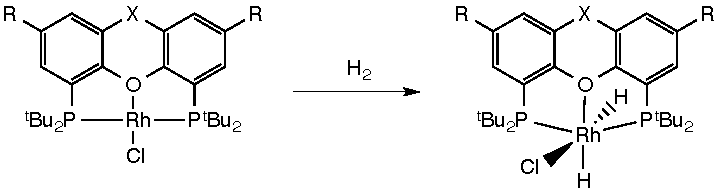
\includegraphics{../Schemes/Rhodiumhydride.pdf}
\caption[Reaction of \ce{[Rh(tBu-xantphos)Cl]} with hydrogen]{Reaction of \ce{Rh(tBu-xantphos)Cl]} with hydrogen.  tBu-xantphos: R = H, X = \ce{CMe2}. tBu-thixantphos: R = Me, X = S. tBu-sixantphos: R = H, X = \ce{SiMe2}}
\vspace{0.2cm} 
\label{Rhodiumhydride}
\end{center}
\end{scheme}
\vspace{0.2cm}

\section{Iridium Complexes}
\label{section:experimental:iridium}

Reaction between \ce{[Ir(COE)2Cl]2} and iPr-xantphos resulted in an iridium(III) complex with the iPr-xantphos coordinating tetradentate through the phosphines, oxygen and a metalled methyl of an isopropyl group.\cite{Esteruelas2013}  Also coordinated are the original chloride ligand and a hydride formed in the metallation.  The reaction likely proceeds via a \ce{[Ir($\eta^3-$iPr-xantphos)Cl]} and then metallation occurs.  However, no spectroscopic evidence for the \ce{Ir($\eta^3-$iPr-xantphos)Cl]} was reported.  Given that metallation occurs on platinum for the reaction between the dioxygen complex and carbon monoxide \fixme{reference} it was expected that metallation should occur in a relatively facile manner when the tBu-xantphos ligands were reacted with \ce{[Ir(COE)2Cl]2}.  

However, when the reactions were carried out they proved to be very slow, and gave intractable mixtures of products.  In each case a large number of hydride resonances were observed indicating that metallation had occurred however, the nature of the complexes was unable to be determined.  The reactions became dark relatively rapidly though they continued to react after this colour change was observed.  The \ce{[Rh($\eta^3-$tBu-xantphos)Cl]} complex was dark red so the colour change is not necessarily a sign of degradation of the iridium starting material.  














